%\documentclass[12pt,a4paper]{article}
\usepackage{xeCJK}
\usepackage{fancyhdr}%页眉页脚
\usepackage{listings}%代码块
\usepackage[margin=1in]{geometry}%页边距
\usepackage{graphics}%图片
\usepackage{fontspec}
\usepackage{amsmath}
\usepackage{amsfonts}
\usepackage{eqnarray}
\usepackage{tabularx}
%定义页眉页脚
\pagestyle{fancy}
\fancyhf{}
\fancyhead[C]{\selectfont \textsc{ACM Template}}
\fancyhead[L]{\rightmark}
\fancyhead[R]{Geometry Rhythm}
%\lfoot{lfoot}
%\cfoot{qkoqhh}
\rfoot{\thepage}
%\renewcommand{\footrulewidth}{0.5pt}

%\rmfamily%罗马字体




\lstset{
	language=C,%代码的语言
	numbers=left,%行号
	frame=single,%
	basicstyle=\footnotesize,
	extendedchars=false,
	basicstyle=\small\ttfamily,
	%	tabsize=2,
	breaklines=true,
	showstringspaces=false
}



\title{ACM Template}
\author{qkoqhh}
%\begin{document}
	\newpage
	\section{博弈}
	\subsection{Turning Tutles}
	\subsubsection{描述}
	Alice和Bob这一次准备玩一个关于硬币的游戏:\\
	N枚硬币排成一列,有的正面朝上,有的背面朝上,从左到右依次编号为1..N。现在两人轮流翻硬币,每次只能将一枚正面朝上的硬币翻过来,并且可以随自己的意愿,在一枚硬币翻转后决定要不要将该硬币左边的任意一枚硬币也翻一次(正面翻到背面或背面翻到正面)。翻最后一枚正面向上的硬币的人获胜。同样的,这次游戏里面Alice仍然先手,两人均采取最优的策略,对于给定的初始局面,Alice会获胜还是Bob会获胜?
	\subsubsection{分析}
	这个游戏叫做Turning Turtles,它的本质就是Nim游戏。\\
	\\
	首先,我们先将局面分解一下,每一次我们只考虑一枚硬币。\\
	不妨设所有硬币全部背面朝上的局面为局面0\\
	假设现在N枚硬币,只有第1枚是正面朝上的。该局面只能转化为全部硬币背面朝上的局面。我们假定该局面为 局面1,则局面1可以转化为局面0。\\
	假设只有第2枚是正面朝上的。该局面可以转化为:只有硬币1正面朝上;全部硬币背面朝上。我们假定该局面为 局面2,局面2可以转化为局面1和局面0。\\
	同理我们可以推定,第i枚硬币正面朝上的局面为局面i,局面i可以转化为局面0..i-1。\\
	\\
	现在,我们考虑把给定的局面拆成单个硬币的局面集合,比如给定了\{HHTHTTHT\},其中H表示正面朝上,T表示背面朝上。那么就是当前局面={局面1,局面2,局面4,局面7}。每一次我们可以改变其中个一个局面,当出现局面0时就从集合中删去。\\
	这样一看是不是就变成了Nim游戏了?然而事实并没有那么简单。\\
	\\
	进一步分析,若同时存在i,j(j<i)两枚硬币正面朝上。我们将这个局面拆成2个单一的局面:即局面i和局面j。\\
	在反转i的时候我们考虑从局面i转移到局面j,那么我们会有两个局面j。\\
	表示第j枚被反转了2次,也就是回到了背面朝上的状态。\\
	那么我们得到这个游戏一个性质:当出现两个同样的局面时,等价于这两个局面合并变成了局面0。\\
	\\
	这种情况在Nim游戏中是没有的,那么它会对Nim游戏的状态造成影响么?\\
	我们想一想,在Nim游戏中,如果出现两个数量相同的堆时,比如A[i]=A[j]。在计算Nim游戏状态时我们采用的xor操作,xor有交换律和结合律。则我们可以变成:\\
	(A[i] xor A[j]) xor Other\\
	因为A[i] = A[j],所以A[i] xor A[j] = 0。上式实际就是:
	0 xor Other\\
	也就是说在原Nim游戏中,若出现了两个数量相同的堆时,实际上这两堆已经不对总局面造成影响了,也就可以认为这两对合并为了一个数量为0的堆。\\
	\\
	到此,我们可以发现这个硬币游戏完全满足Nim游戏的规则,其解答也满足Nim游戏的性质,这题也就很简单的转化为了普通的Nim游戏。在实际的博弈游戏中会发现很多都是可以转化为Nim游戏模型。如何正确的建立模型和转化游戏模型也就是解决博弈游戏一个很重要的手段。
	\newpage
	\subsection{阶梯博弈}
	\subsubsection{描述}
	从\textbf{第0个阶梯}起,每个阶梯上都有若干个石子,每次都可以从任一阶梯上取任意正整数个石子往下一个阶梯放,不能操作的人输
	\subsubsection{结论}
	该状态的sg值为奇数阶梯上的石子的异或和
	\subsubsection{分析}
	先证明这个模型可以转化为把奇数阶看成若干堆石子的nim博弈\\
	如果对手从偶数阶往奇数阶放,那么我们可以从该奇数阶取相同的石子到下一阶,即将偶数阶的石子放到了下一个偶数阶,此时奇数阶的状态数不变\\
	如果对手从奇数阶往偶数阶放,相当于把奇数阶上的石子拿掉了,此时可以根据nim博弈取相应的石子到达sg=0的状态\\
	于是这个阶梯博弈就看成了奇数阶上的nim博弈,其sg值自然也是奇数阶上的石子数的异或和\\
	\newpage
	\subsection{Green Hackenbush}~
	
	Hackenbush游戏是通过移除一个有根图的某些边,直到没有与地板的相连的边。地板用虚线来表示,其中移除某一条边的时候,那条边以上所连着的所有边都会移除,就像砍树枝那样,树枝以上的部分也会被移除。
	
	在这节中,我们讨论这个游戏的公平版本,每个玩家在他的回合可以删除任意的边。这个版本叫做Green Hackenbush,每条边都是绿色的,下面我们简称GH游戏。这里还有一个不公平版本,叫做Blue-Red Hackenbush,有些边是蓝色,有些边是红色,而玩家一只能删除蓝色边,玩家二只能删除红色边。总的来说,Hackenbush游戏,可能会有只供玩家一删除的蓝色边,只供玩家二删除的红色边,还有两个玩家都可以进行操作的绿色边。
	~\\
	\subsubsection{Bamboo Stalks}~
	
	作为GH游戏的介绍,我们先研究下面的 Figure 6.1。n条线段的bamboo stalks游戏是具有n条边的线形图。一步合法的操作是移除任意一条边,玩家轮流进行操作,最后一个进行操作的玩家获胜。n条线段的bamboo stalks游戏能够移动到任意更小线段数(0到n-1)的bamboo stalks游戏局面当中。所以n条线段的bamboo stalks游戏是等同于nim游戏中其中拥有n个石子的一堆。玩一组bamboo stalks游戏就相当于玩nim游戏。
	\begin{center}
	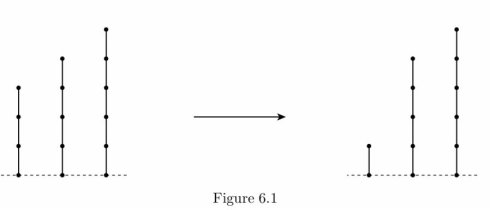
\includegraphics{./source/img5.jpeg}
	\end{center}
	
	例如,左边的三根竹竿构成的“森林”相当于具有石子数分别为3、4、5三堆石子的nim游戏。就我们所知,$3\oplus4\oplus5=2$,这是一个能够移动到P局面的N局面,办法是通过取走三根线段的竹竿上的第二根线段,留下一根。而结果变成右边的竹竿分布,而此时的SG值是0,是P局面。
	~\\
	\subsubsection{Green Hackenbush on Trees}~
	
	通过bamboo stalks游戏,我们知道GH游戏是换了个形式的nim游戏而已。可是如果我们允许比bamboo stalks游戏更多结构呢?让我们看下在Figure 6.2中由三棵根树组成的森林。根树是一种图,带有一个最高的节点,叫做根,这个根到任意一个其他节点的路径都是独一无二的。实质上就是说这个图不含有圈。
	\begin{center}
	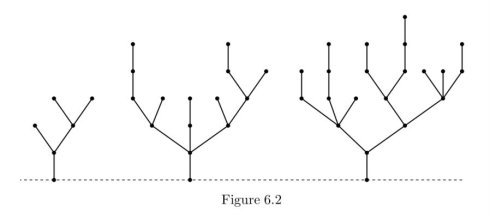
\includegraphics{./source/img6.jpg}
	\end{center}
	
	一次合法操作是移除任意一条不与地面相连的线段,此时次线段以上的子树都会被移除。既然这个游戏是公平的,而且根据我们学过的nim游戏,这样的树相当于nim游戏的一些堆,或者说是bamboo stalks游戏(到了这里明白bamboo stalks游戏与nim游戏的单堆是等价的)。这个问题就是寻找每棵树的SG值。
	
	这里我们要用上一个原理,叫做\textbf{Colon Principle}:当树枝在一个顶点上时,用一个非树枝的杆的长度来替代,相当于他们的n异或之和。
	
	让我们看看这条原理是如何在Figure 6.2中寻找与左树等价的竹竿。这里有两个节点拥有树枝。较高的那个节点拥有两个树枝,每个树枝上有两个节点。$1\oplus1=0$,所以这两个树枝可以用一个带有0个节点树枝来代替,也就是说可以把这两个树枝给去掉。那就剩下了一个Y形树了,因为同样道理这个Y形树的两个树枝也要被去掉。此时就剩下了一个线段数为1的竹竿游戏模型了。
	
	看Figure 6.3,是Figure 6.2中第二棵树的处理办法,最后可以得到线段数为8的竹竿游戏。第三棵树也可以同样处理,结果是线段数为4的竹竿游戏。(注意,这里所指的竹竿游戏都实质上是nim游戏中的单堆石子)
	\begin{center}
	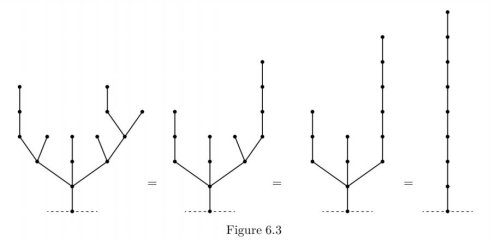
\includegraphics{./source/img7.jpg}
	\end{center}
	
	现在我们可以计算一下图6.2三棵树的sg值,也就是 $1\oplus8\oplus4=13$.既然这个SG值不为0,那么就是一个N局面,先手必胜。问题是要怎么找到胜利方法。很明显这里有一个必胜移动,通过将第二棵树进行操作使得它的SG值为5.可是我们要找哪条边呢?
	
	Figure 6.3的最后一个树长度是8,因为它的前一棵树的三个树枝长度分别是3,2,6,异或值为 $3\oplus2\oplus6=7$,用长度为7的竹竿代替三个树枝后,树的长度就是根加上竹竿长度,即1+7=8。为了最后SG达到5,即使树的长度为5,我们要用长度为4的竹竿来替代那三个树枝。因为 $2\oplus6=4$,所以我们只要将最左边的树枝去掉就行了,当然我们也可以将树枝改动成 $3\oplus1\oplus6=4$.
	
	修剪树的方法用冒号给出了,把所有的树化简为一个单一的竹竿。一个从最高的树枝开始,然后用原理归纳往下到根部。我们现在展示这个原理对于含圈和多重根边的图同样适用。
	\paragraph{Colon Principle的证明}假设一个任意固定的图G,一个任意节点x,让H1和H2为任意的树,且拥有相同的SG值。考虑这样两个图G1=Gx:H1和G2=Gx:H2,Gx:Hi表示该图是把树Hi连接图的x节点。Colon Principle阐述的是两个图G1、G2拥有相同的SG值。看看Figure 6.4的两个游戏。\\
	G1、G2拥有相同的SG值意味着两个游戏的总SG值为0,G1+G2的和是一个P局面,也就是必败
	\begin{center}
		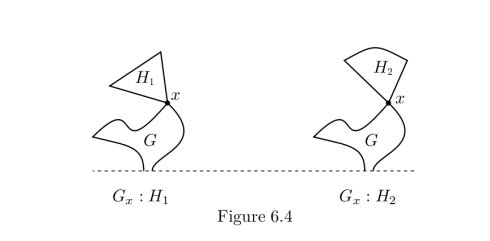
\includegraphics[scale=0.7]{./source/img8.jpg}
	\end{center}
	
	先手一旦在其中一幅图中取走任意一条边,后手即可在另一幅图中取走相同的一条边。轮流下去,最后肯定是后手获胜。所以当树枝在一个顶点上时,用一个非树枝的杆的长度来替代,二者的结果是等价的。
	
	~\\
	\subsubsection{Green Hackenbush on general rooted graphs}~
	
	现在让我们来考虑不规则的图。这些图可能会有圈,会有几条根。看Figure 6.5.
	\begin{center}
		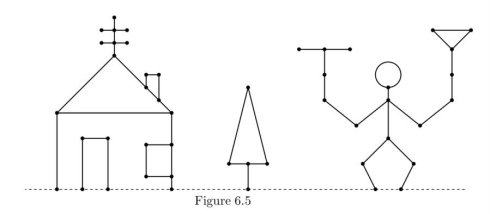
\includegraphics{./source/img9.jpg}
	\end{center}
	
	同样,上面的三个图,每个图都相当于nim游戏的一个堆,三个图组成了一个nim游戏。接下来我们要找到这些图等价的nim堆,方便我们解决问题。这要用到融合原则。我们可以把两个相邻的节点合成一个节点,并把它们之间的边弯曲,变成一个圈。一个圈是把自己作为边的另一端的一种边。比如Figure 6.5的最右边那个杂戏表演者的头就是一个圈。在GH游戏中,一个圈是可以被一个叶子(一条没有任何树枝与它相连的边)所代替的,见Figure 6.6中第三幅图到第四幅图的转化。
	
	The Fusion Principle:任何环内的节点可以融合成一点而不会改变图的sg值。(下面我们称它为融合原则)
	
	融合原则允许我们把任意一个根图简化为一个等效的可以通过冒号原则(即Colon Principle)简化为竹竿的树。
	
	如下图左部分所示的一个门,在地板上的两个节点是同样的节点来的(记住地板相当于一个单独的节点),所以实际上是一个有一个节点与地板相连的三角形,即第二幅图。融合原则告诉我们,这相当于一个单独的节点有三个圈与它相连。所以造就了第三幅到第四幅的转变,过程是把任意两点收缩成一个圈,3个点两两收缩便可得到三个圈。每个圈又相当于长度为1的竹竿,它们的异或和还是长度为1的竹竿。
	\begin{center}
		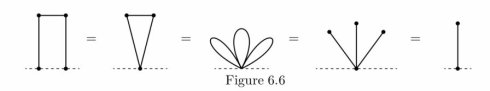
\includegraphics{./source/img10.jpg}
	\end{center}
	
	我们会发现,拥有奇数条边的环可简化为一条边,偶数条边的环可简化为一个节点。例如,在Figure 6.5中的第二幅图圣诞树中的有四条边的环,会缩减成一个节点,所以这圣诞树最后会简化为一个长度为1的竹竿。相似的,房子上的烟囱变成一个单独的节点,右边的窗户变成一个点,继续下去,就可以看出房子的SG值为3。
	
	融合原则的证明比冒号原则的证明更长,所以在此不做解释。
	\begin{center}
		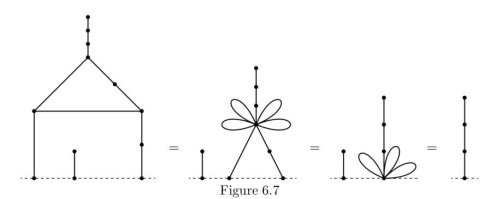
\includegraphics{./source/img11.jpg}
	\end{center}
	~\\
	附注:\\
	本文译自《Game Theory》,由于这篇文章是译文,语言上可能有些不恰当,下面做些补注。\\
	GH游戏:即 Green Hackenbush,这篇文章探讨的博弈游戏。\\
	竹竿游戏:即Bamboo Stalks,是直译过来的。\\
	冒号原则:即Colon Principle,这个虽然是直译,可是不太好,有保留。\\
	融合原则:即Fusion Principle\\
%	\newpage
%	\subsection{}
%	\lstinputlisting{./source/}
%\end{document}